% Ein Beispielkapitel
%

\chapter{Implementation}

The program and modules developed in this thesis enables the building and simulation
of a full mouse brain model relaying on point neuron models. Such a model must be build by
reconstructing parts of the model from experimental data.
Allen Institute for Brain for Science and the Blue Brain Project provide such data.
To this aim, the pipeline of large scale data-driven simulations with the NEST simulator is investigated.
An efficient data format is defined, the circuit generation scripts are adapted to
run on a bigger scale and the NEST simulator is extended to load the new data format.

\section{Data formats}
\label{sec:dataformats}
A point neuron model contains point neurons and connections (synapses) between the point neurons.
The same point neuron model (conductance based exponential integrate-and-fire neuron model \cite{brette2005adaptive}) and synapse model (Tsodyks synapse model containing synaptic short-term depression and short-term facilitation \cite{tsodyks1997neural, fuhrmann2002coding}) are used for all neurons and synapses respectively.
The neurons and synapses are characterized by parameters.
Each neuron is defined by a given set of parameters.
Besides the parameters, the synapses contain pre-synaptic and post-synaptic neuron ids.
To store the circuit in files two different data formats are defined.
The first data format defines the storage for all neuron parameters.
The second data format defines the storage for synapse parameters and pre-synaptic and post-synaptic neuron ids.

The data format for the neurons and the synapses follow two different concepts.
The neuron data format contains multiple datasets containing the neuron parameters.
All datasets have by definition the same length. This length defines the number of neurons.
The neuron parameters of neuron $i$ are stored in the i-th line of each dataset.
\begin{figure}[ht!]
   	\begin{center}
        \subfigure[The neuron file contains a dataset for each parameter.
        Each dataset is a one dimensional array of \emph{H5T\_NATIVE\_FLOAT} values.]{%
            \label{fig:allInjections}
            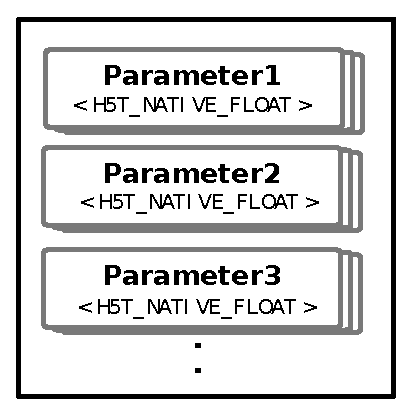
\includegraphics[scale=0.5]{pictures/hdf5_neuron_format.eps}
        }
        \hspace{1cm}
        \subfigure[The synapse file contains two datasets: \emph{neuron} and \emph{syn}.
		\emph{neuron} groups the pre-synaptic neuron ids with references to the \emph{syn} dataset.
		\emph{syn} contains post-synaptic neuron ids and synapse model parameters.]{%
            \label{fig:oneProjection}
            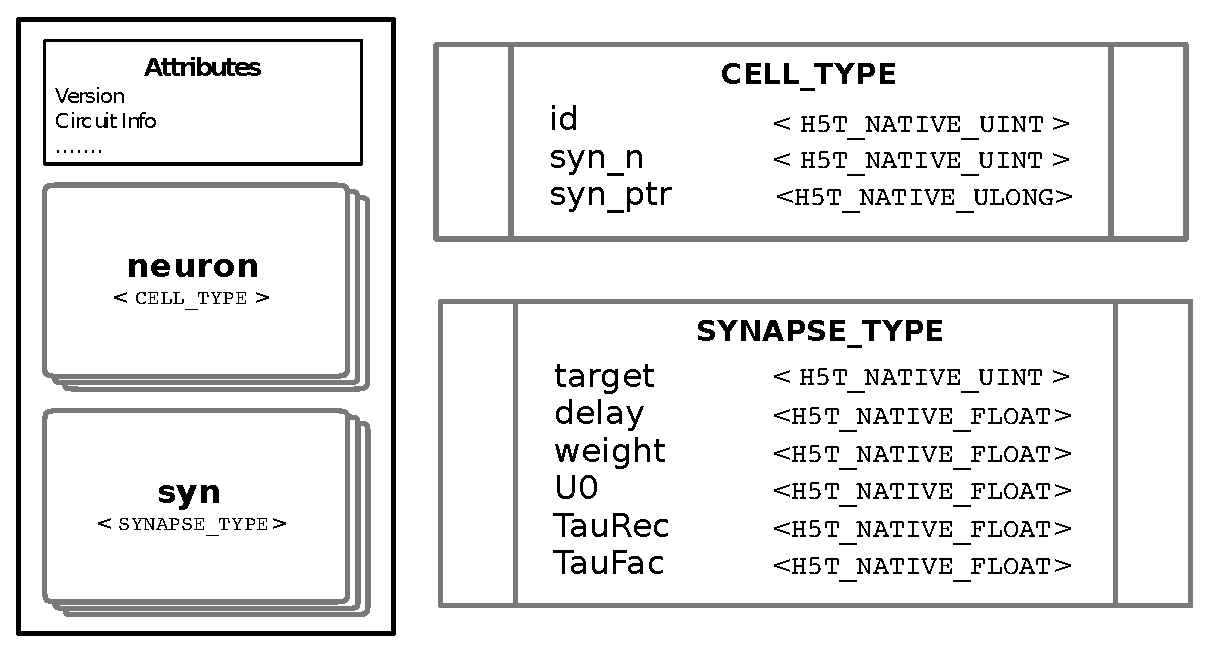
\includegraphics[scale=0.41]{pictures/hdf5_syn_format.eps}
       }
    	   \end{center}
    	\caption{%
        The diagram shows the data format with the related datasets and data types.
     }%
   \label{fig:atlas}
   \end{figure}
   
The synapse data format contains two datasets. In general the datasets contain for each synapse
a pre-synaptic neuron id, a post-synaptic neuron id and a set of parameters.
To reduce the amount of data the pre-synaptic neuron ids are grouped together in one \emph{neuron} dataset.
This is feasible, because
the number of synapses is way bigger than the number of pre-synaptic neurons ($~11,000$ synapses per pre-synaptic neuron).
The dataset contains an array of  pre-synaptic neuron ids (\emph{id}) with references (\emph{syn\_n} and \emph{syn\_ptr}).
The \emph{syn\_ptr} value defines the related starting index in the \emph{syn} dataset,
and \emph{syn\_n} defines the number of related following entries.
The \emph{syn} dataset contains the post-synaptic neuron id and a set of parameters.
Both datasets use a compound data type to store different data types in the same dataset.

\newpage
\section{Circuit generation}
The already existing python scripts can generate circuits up to one percent of the full mouse brain model.
The scripts are developed to fit on local laptops.
Going the way towards the full mouse brain model, larger machines have to be taken into account.
A full mouse brain model generation requires more resources and computation power.
Therefore the circuit generation should be ported to the Blue Brain IV super computer.
A new implementation should make use of the available resources.
Rewriting the sequential python scripts to a hybrid C++ application requires a parallel implementation of the algorithms.


%%insert somewhere
%Unfortunately all injections from these experiments do not
%cover the whole brain. So there are neurons which are not injected
%by any experiment. Therefore all neurons which are not injected should use the projection
%from the nearest injection.


\subsection{Long range connections}

The sequential long range connections generation algorithm (see Algorithms \ref{}) is mainly based on three nested for loops.
The outer one iterates over the experiments, the next inner one over voxels, which are injected by the experiment and the third
one over neurons inside the voxel.
Besides a if condition in the voxel iteration, there are no dependencies between the iterations.
The if condition compares the total injection densities.
It only regenerates the connections for the voxel, if the current
experiment injects less than the previous experiments (less injection means more precise projections).
For a parallel implementation this dependency has to be avoided.
To overcome the dependency, the best chosen experiment (the best experiment per voxel is the experiment with the smallest injection which still injects the current voxel) per voxel is calculated beforehand.
Thus the loop over the voxels moves outside the loop over the experiments.

When the used voxels are identified the number of generated synapses can be calculated, based on the
number of neurons inside the voxels and the hard-coded number of synapses per neuron.
Thus the HDF5 file and the \emph{syn} dataset is created before the voxel iterations.
The iterations of the loop over the voxels are distributed on the processes.
Inside the iteration over all neurons the sequential algorithm can be applied.



Figure \ref{fig:longrangParallel} illustrates the workflow of all processes.
\begin{figure}[ht!]
\centering
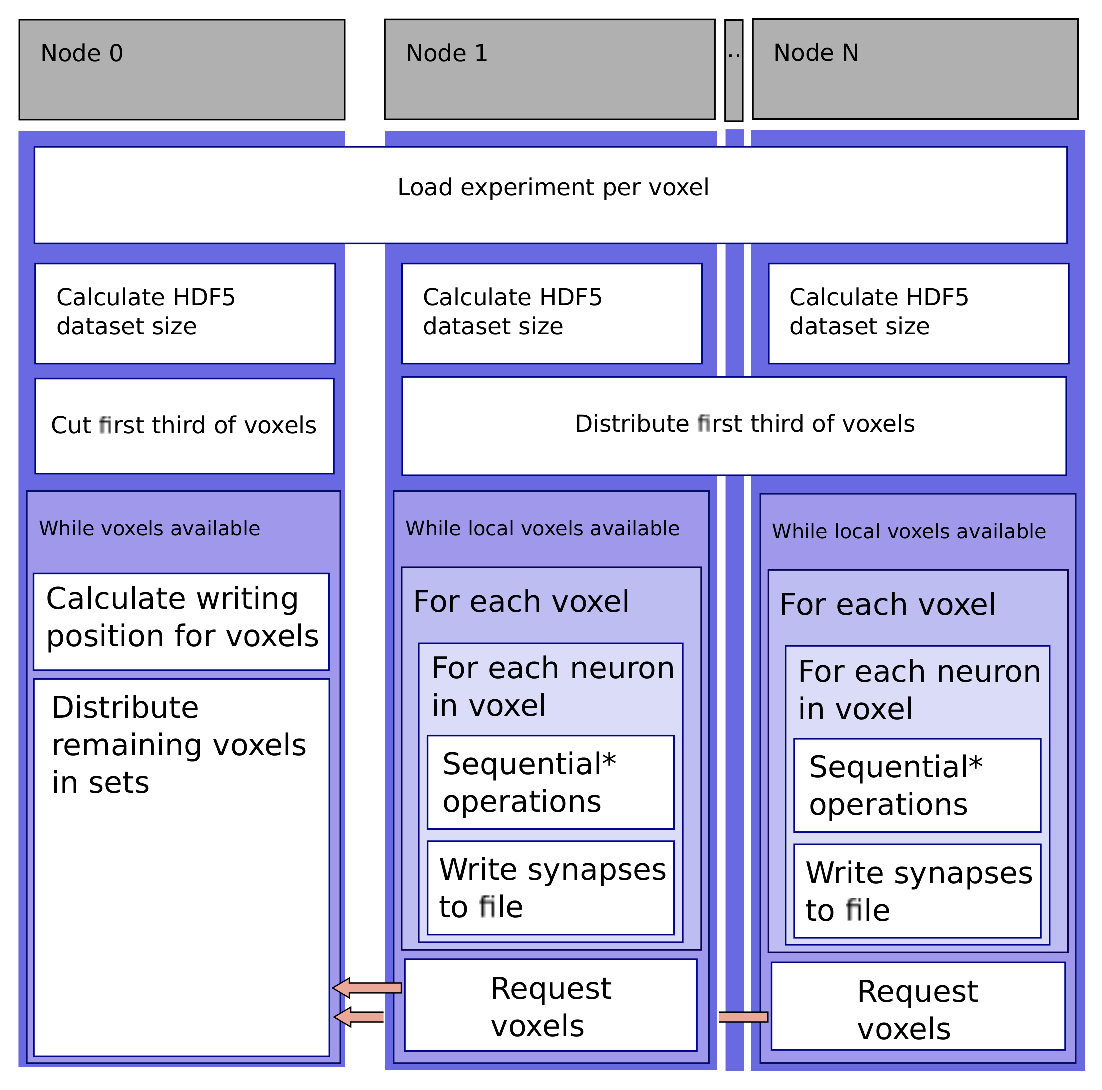
\includegraphics[scale=0.5]{pictures/longRange_parallelAlg.eps}
\caption{Task distribution between the processes for the long range connections generation. It illustrates which tasks are distributed between which processes.}
\label{fig:longrangParallel}
\end{figure}
\emph{Process 0} is selected as the master process. It does not participate on the iterations.
It manages the dynamic distribution of the voxels to the other processes and 
assigns write positions to each voxels. Thus each process receives besides the 
voxel information the positions,
where it has to write its data to the HDF5 datasets.
\begin{figure}[ht!]
\centering
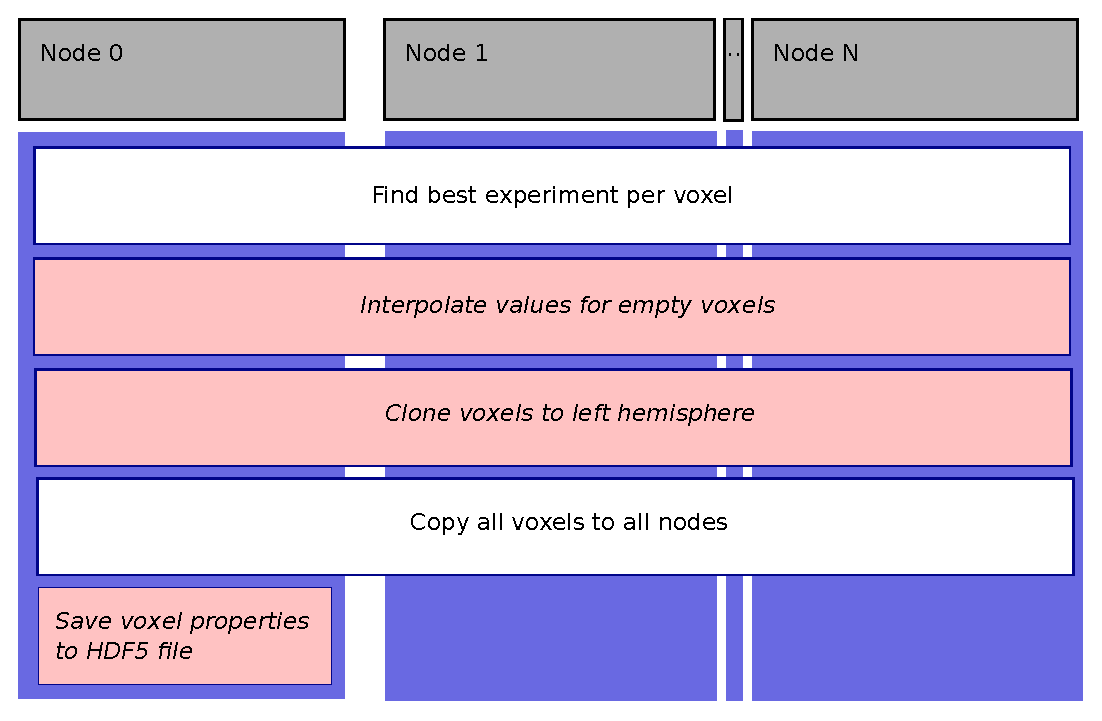
\includegraphics[scale=0.5]{pictures/longRange_BestExp_parallelAlg.eps}
\caption{Subtasks of the above listed \emph{Load experiment per voxel} task}
\label{fig:longrangeLEPV}
\end{figure}
Task \emph{Load experiment per voxel} from Figure \ref{fig:longrangParallel} contain several subtasks.
It generates the voxel datasets, which are distributed afterwards.
Manipulations of the generation effect mostly this part.
So the part allows modifications of the applied functionalities. 
Further the whole function can be skipped by loading the voxel information from file \ref{file:voxelinfo}.
Figure \ref{fig:longrangeLEPV} shows the subtasks.
The red tasks are optional and can be activated via command line arguments.
In the first task \emph{Find best experiment per voxel} each process loads a set of experiments.
Iteratively the experiment with the smallest total injection density is assigned to each voxel
on each process. Afterwards a MPI reduction function returns the smallest value for each voxel on
each process.
But there are regions which were not injected by any experiment available.
So there is no connection information available for the internal neurons.
To overcome the missing data a piecewise constant interpolation is applied to the chosen experiment per voxel
in \emph{Interpolate values for empty voxels} (see paragraph \ref{par:interpolation}).
Afterwards the voxels are mirrored from the right to the left hemisphere, because the
Allen Brain Atlas mostly delivers injection sites for the right hemisphere and
the mouse brain model is assumed to be symmetric.
Finally all voxel information are gathered to all processes.
For debugging or manipulating purposes, task \emph{Save voxel properties to HDF5 file} can be used
to save the generated voxel information to file (see chapter \ref{file:voxelinfo}).

Finally, the first third of the voxels are distributed (see paragraph \ref{par:loadbalancing}) on the processes.
Each process iterates over its voxels and generates connections for each neuron inside the voxels.
Therefore the sequential algorithm is used.

\paragraph{Linear acceptance rejection optimization}
\label{par:linearacceptancerejection}
Further optimization are applied to the linear acceptance rejection function,
which picks the neurons in the projection area.
In the given sequential algorithm each neuron has its own probability.
But as given by the assignment all neurons in each voxel have the same value.
So at first a target voxel is selected and afterwards a neuron is picked from the chosen voxel.
To make use of all cores in the linear acceptance rejection function
(it picks the post-synaptic neurons and takes most of the computation time per iteration)
distributes its internal loop on the available threads.
Each thread picks $~ \frac{10,000}{N_{threads}}$ post-synaptic neurons.
In the end of each iteration each process writes its generated connection independently to file.

%\begin{figure}[ht!]
%   	\begin{center}
%        \subfigure[All nodes are equal and process the work based on a static distribution]{%
%            \label{fig:shortColumn}
%            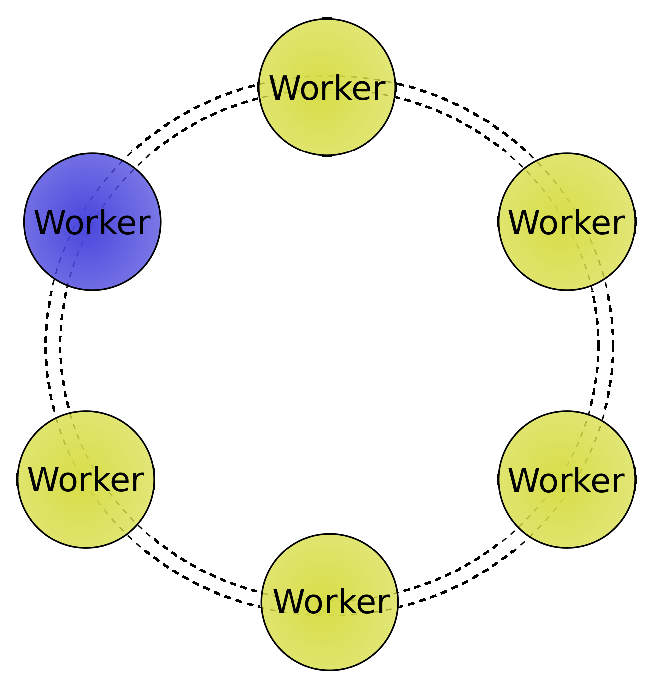
\includegraphics[scale=0.5]{pictures/All_Worker_Collective.eps}
%        }
%        \hspace{1cm}
%        \subfigure[The 0 node is assigned as the master node and handles from this on the management of the work distribution.]{%
%            \label{fig:shortColumnInCircuit}
%            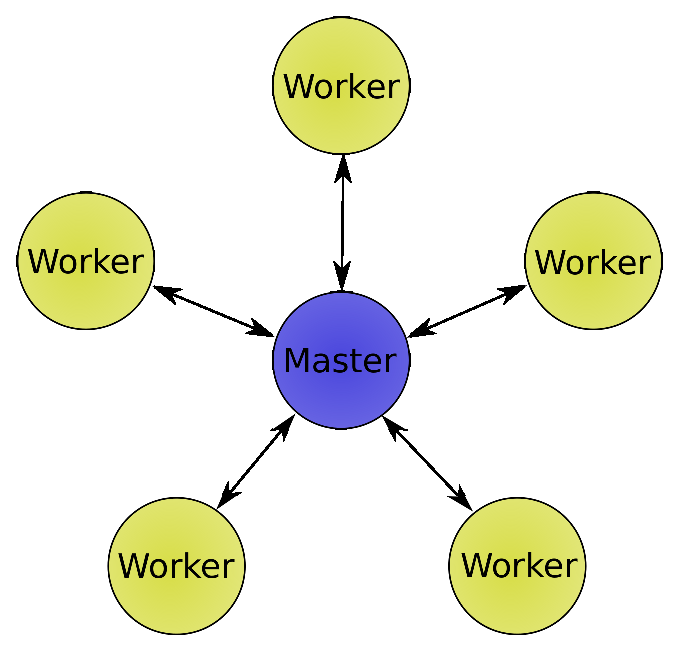
\includegraphics[scale=0.5]{pictures/MasterWorker.eps}
%       }
%    	   \end{center}
%    	\caption{%
%        The figure illustrates the work distribution and communication between the nodes.
%     }%
%   \label{fig:atlas}
%   \end{figure}

\paragraph{Load balancing}
\label{par:loadbalancing}
An efficient parallel implementation depends on the distribution of the voxels.
The work load should be distributed equably on all processes.
Therefore an estimation of the work load per iteration is necessary.
But it \ref{eq:L} depends on the properties of the given neurons.
The iterations can be partitioned into five parts: acceptance rejection method (\emph{linear}), storing to disk (\emph{store}),
loading experiment data (\emph{load}), select neurons in injection (\emph{selI}), select neurons in projection (\emph{selP}).
\begin{equation} \label{eq:L}
	L \approx L_{linear}(n,m,M) + L_{store}(n,\omega) + L_{load}(\nu) + L_{selI}(n) + L_{selP}(m,\nu)
\end{equation}
$L_{load}(\nu)$, $L_{selI}(n)$ and $L_{selP}(m,\nu)$ are neglectable.
$\Omega$ and $\frac{\partial L_{linear}(n,m,M)}{\partial M}$  can not be estimated satisfyingly.
$\Omega$ represents waiting times, which occur from independent parallel write operations.
$M$ represents the distribution of probability values.
The distribution effects the number rejections inside the linear rejection method.
Therefore it has a significant impact on the wall-clock time.
Thus there is only a rough estimation of the wall-clock time per voxel iteration possible.
\begin{equation} \label{eq:Lapprox}
	L_{estimate} = L_{linear}(n,m) + L_{store}(n)
\end{equation}
Therefore a statically and dynamically voxel distribution is implemented.
At first a third of all voxels are distributed (using algorithm \ref{alg:distributeWeightedVoxels}) based on the weight $L_{estimate}$ \ref{eq:Lapprox}  per voxel.
\begin{algorithm}[ht!]
\KwData{List of all voxels with weights}
\KwResult{List of private voxels and sum of weights per process}
\For{voxel n}{
	Find Process with smallest sum of weights \\
	Add weight to sum of weights of Process \\
	\If{Process is me}{
		Add voxel to private voxel list
	}
}
\caption{Algorithm to distribute weighted voxels to processes}
\label{alg:distributeWeightedVoxels}
\end{algorithm}
After that the master process distributes further voxels in sets on request from the other processes.

\paragraph{Interpolate connection information}
\label{par:interpolation}

The constant interpolation of connection information, interpolates the used experiment per voxel in 3D space.
It is realised with an iteratively nearest neighbour search algorithm for each missing voxel.
The algorithm iterates over all neighbours with increasing distance.
Figure \ref{longrange} shows an illustration of the search algorithm
projected in a 2D plane.
\begin{figure}[ht!]
\centering
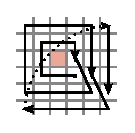
\includegraphics[scale=2.5]{pictures/longRange_Nearest_parallelAlg.eps}
\caption{Find nearest neighbour loop}
\label{longrange}
\end{figure}
The first voxel along the search direction which is found is declared as the nearest neighbour.
The chosen experiment from the nearest neighbour is adopted.



\subsection{Short range connections}

The short range connection generation algorithm \ref{alg:BBP} presented in the analysis section can be parallelized straight forward.
Each iteration is independent. Number of synapses which are created is not know. It is available
at the end. Therefore all synpases are stored inside of memory during the iterations and only written to disk 
at the end.

\begin{figure}[ht!]
\centering
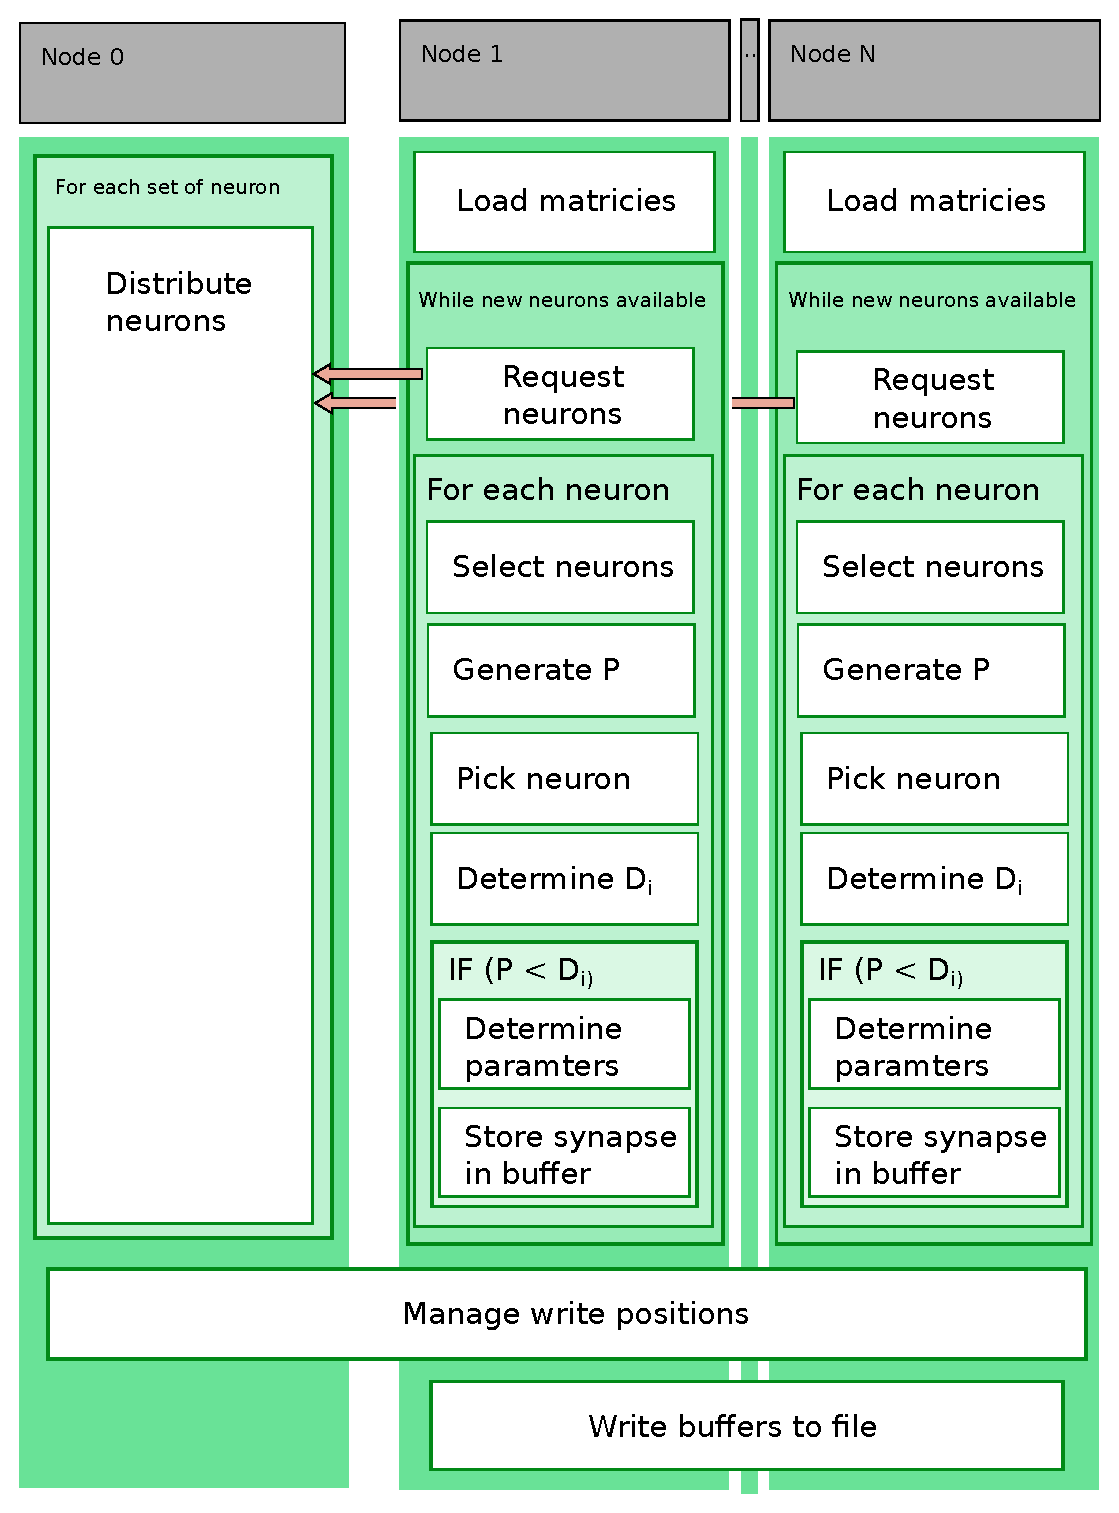
\includegraphics[scale=0.5]{pictures/shortRange_parallelAlg.eps}
\end{figure}

The iterations from the main loop from the sequential algorithm \ref{alg:BBP} are distributed between the processes.
The short range algorithm follows the same concepts as the long range generation parallelization.
The iterations are distributed first statically and afterwards dynamically.
The master process, \emph{Process 0}, handles the dynamic distribution management.
To overcome that the dynamical distribution becomes a bottleneck in the beginning a third of the iterations are distributed
statically between the working processes beforehand.
The work-load per neuron is not estimated in advance.
The iterations are partitioned continuously without weights.
Each process of the workers (all processes except of \emph{Process 0}) receives the neurons with the ids $x_{process\_id-1}$
to $x_{process\_id}$ (\emph{Process 0} is not part of distribution. It is skipped.).
$x_i$ relates to equation \ref{eq:process2id}.
\begin{equation}
	x_i = round(i * \frac{N_{neurons}}{N_{processes}-1})
	\label{eq:process2id}
\end{equation}
During runtime the master process manages the distribution of the neurons. For each neuron 
outgoing synapses have to be created. In the first step, the workers load all needed matrices from the file system.
Then each process request a set of neurons from the master process. Over this set it iterates and creates resulting
synapses. The library Random123 is used to get values for the random variable. Therefore a parallel usage of 
the given sequential algorithm is possible. Only the storage of the generated synapse list, has to be done 
after all iterations. So in each loop the synapse list is stored in a buffer.
The buffer is based on an own implemented queue class. It nests standard vectors.
It contains one vector of fixed size vectors, which contain the synapse objects.
The buffer size is adapted to 
the memory available on the used Blue Gene Q systems.
The buffer is written to disk in chunks (sub vectors). The sub vectors are
accessible and can be written as chunks to file.
When all neurons are distributed and processed, all processes, including the master process, calculate the writing position
in the HDF5 datasets where each process has to write its data to. After that all workers write theirs synapse vectors to
disk.


%\begin{figure}[ht!]
%   	\begin{center}
%        \subfigure[Master-worker strategy to get good balance properties]{%
%            \label{fig:shortColumn}
%            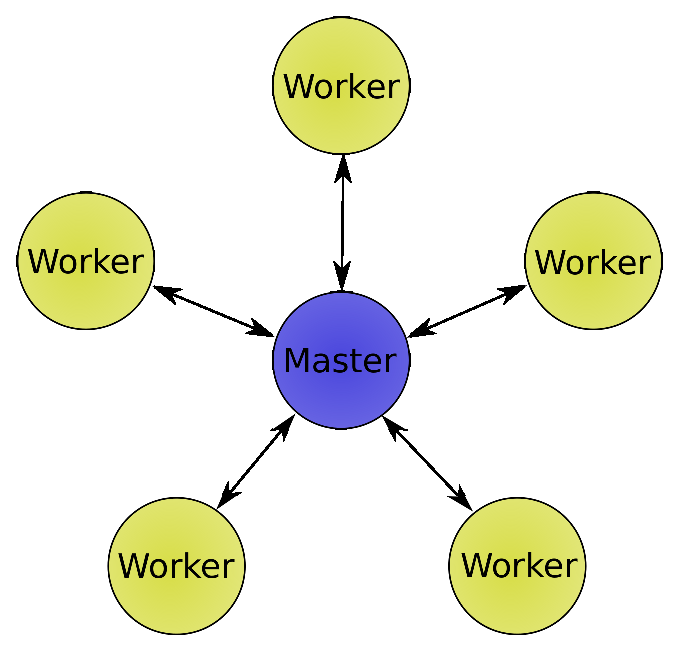
\includegraphics[scale=0.5]{pictures/MasterWorker.eps}
%        }
%        \hspace{1cm}
%        \subfigure[Collective write operation to maximize used bandwidth]{%
%            \label{fig:shortColumnInCircuit}
%            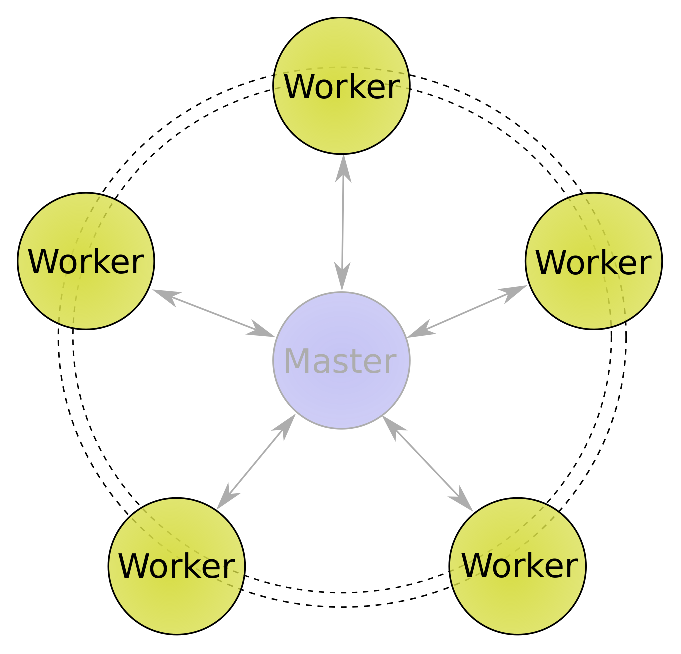
\includegraphics[scale=0.5]{pictures/Worker_Collective.eps}
%       }
%    	   \end{center}
%    	\caption{%
%        The figure illustrates the work distribution and communication between the nodes.
%     }%
%   \label{fig:atlas}
%   \end{figure}


\newpage
\section{Circuit validation}
In the context of this thesis the circuit is validated in terms of geometrically correct placement of
the synapses. The position of the pre-synaptic and post-synaptic neurons can be visualized and  compared to a 
reference system. For the long and the short range connectivity the geometrical shape is know.
In particular the long range connectivity should connect neurons from the injected regions to neurons
in the projected region for each experiment. Therefore a circuit for a single experiment is 
generated, the pre-synaptic and post-synaptic neurons are visualized in a 3D coordinate system and the the injection
and projection is used as the reference system. If source neurons are inside the injection space and all
post-synaptic neurons are in the projection space, the implementation is correct.
For the short range connectivity all post-synaptic neurons connected via synapses to the same pre-synaptic neuron should
lay inside a cylinder in layer 1 to 6. Visualising the post-synaptic neuron placement on top of the contour of layer 1 to 6 allows to review if the shape matches with a cylinder.
To perform the validation the renderer voxalize \ref{sec:voxelize} is used.
It reduces the post-synaptic neuron cloud to densities of neurons per voxel ($N_{x,y,z}$).
The voxels can be directly compared to the projection densities ($P_{x,y,z}$) from an experiment.
\begin{equation}
	P_{x,y,z} \propto N_{x,y,z}
\end{equation}
The relation between the densities should be proportional.
The visualization tool Paraview \ref{paraview} allows a visual comparison of the density values.
 \begin{figure}[ht!]
\centering
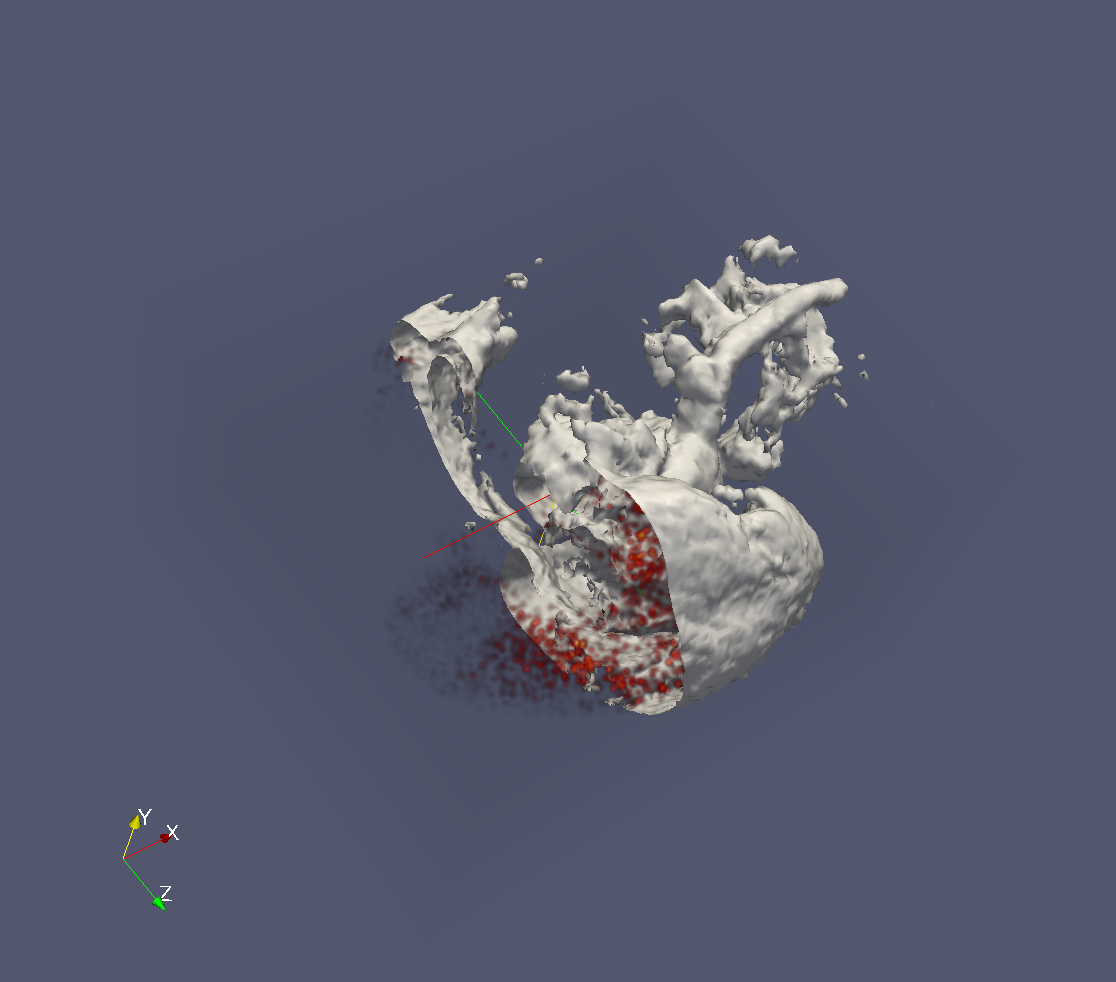
\includegraphics[width=0.4\textwidth]{pictures/paraview_ex.png}
\end{figure}
For a visual validation the Blue Brain Project visualization team offered a rendering pipeline to visualize the placement of post-synaptic neurons for each synapse file. Therefore the neuron and synapse files can be imported into 
Voxelize \ref{sec:voxelize}. Voxelize creates a voxelized dataset out of the post-synaptic neuron positions, which can be exported into
a MetaImage \ref{sec:MetaImage} file or directly viewed with Livre \ref{sec:livre}.
The MetaImage files can be viewed with Paraview \ref{sec:paraview}.
Injection and projection images are also given in the MetaImage format.
A direct comparison inside of Paraview is possible.
Loading the projection inside of Paraview and applying the contour filter on it with a threshold of $0.01$ (threshold is also applied to the same data in the long range connectivity generation) allows to visualize the valid boundaries for all post-synaptic neurons for this particular experiment.
 
\begin{figure}[ht!]
   	\begin{center}
        \subfigure[Densities in 3D space of the projection]{%
            \label{fig:allInjections}
            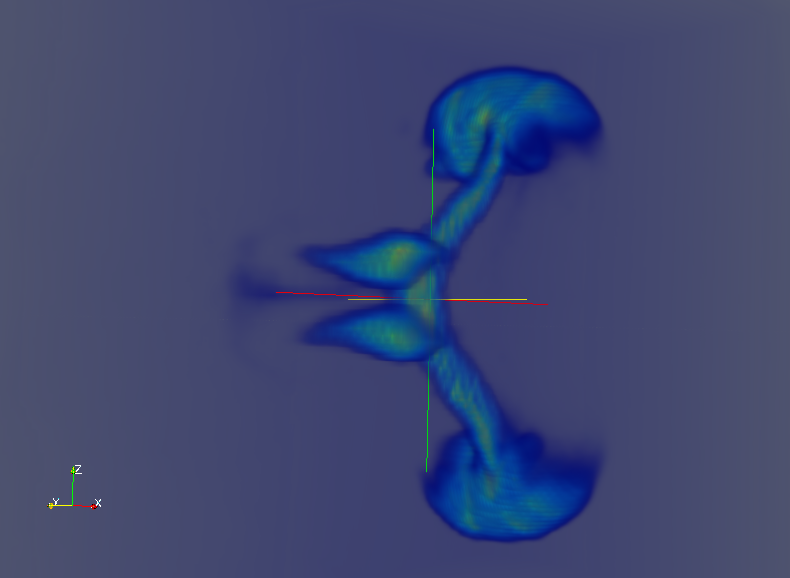
\includegraphics[scale=0.15]{pictures/exp1_energy.png}
        }
        \hspace{0.2cm}
        \subfigure[Post-synaptic neuron placement in 3D space]{%
            \label{fig:oneProjection}
            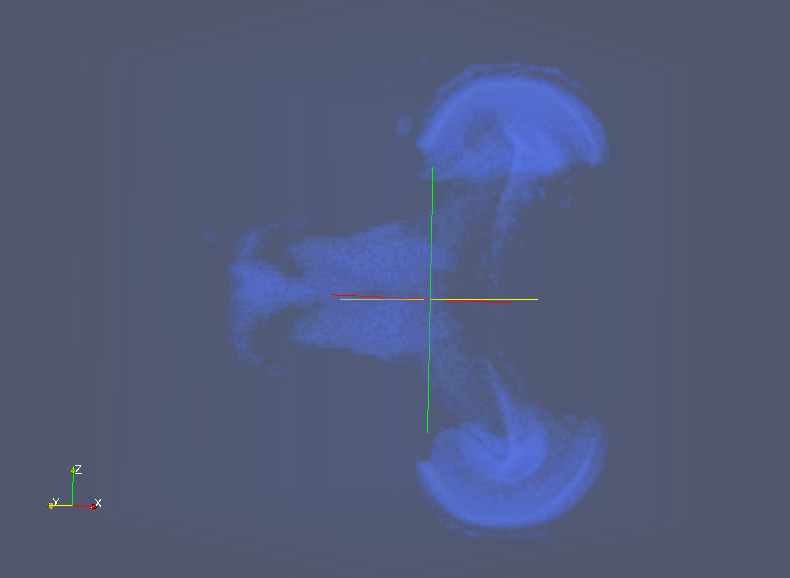
\includegraphics[scale=0.15]{pictures/exp1_post.png}
       }
       \hspace{0.2cm}
        \subfigure[Post-synaptic neuron placement inside of half cutted contour of the projection densities]{%
            \label{fig:oneProjection}
            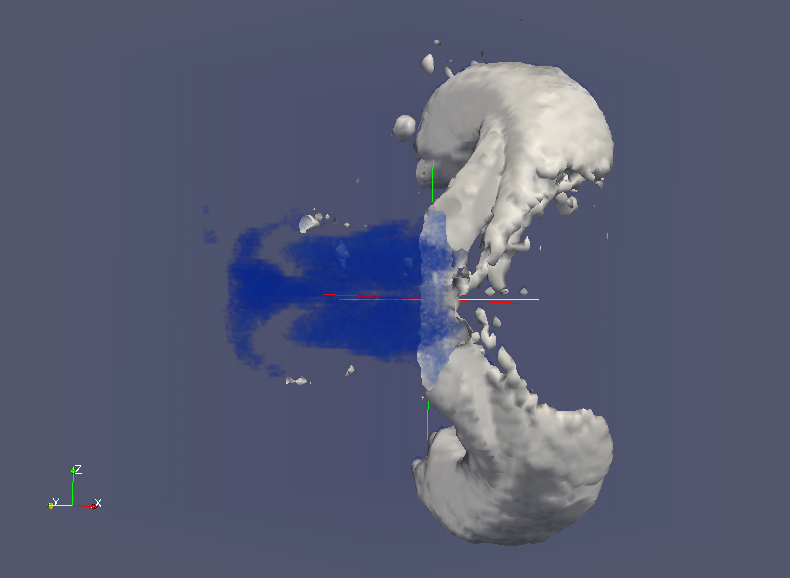
\includegraphics[scale=0.15]{pictures/exp1_post_contour.png}
       }
    \end{center}
    	\caption{%
        Example of visual long range connections validation of a single experiment (id: 113935285).
        The used connections are part of the full circuit.
     }%
   \label{fig:longrangevalidation}
   \end{figure}
   
The example \ref{fig:longrangevalidation} illustrates the usage of the visual validation of long range connections.
It shows that for the specific experiment the post-synaptic neurons are placed inside the correct regions.

\section{NEST import modules}
The neuronal spiking network simulator NEST is developed in \emph{C++} and delivers
a user interface based on its own description language \emph{SLI} and a Python interface.
The large scale data-driven simulation use case shall be integrated into the standard work flow of NEST.
To this end, the functionality in \emph{C++} the interfaces have to be extended.
The difficulties of the network building inside of NEST is based on a difference in 
the NEST internal data structure and the data delivered by the circuit generation.
Connection information contains pre-synaptic and post-synaptic neurons besides biochemical
information of the synapses. Because of the in vitro injection methods the
connection information maps the synapse from the pre-synaptic to the post-synaptic neurons.
For multi process simulations NEST distributes all neurons based on a modulo function 
to the processes. Because of memory optimizations the synapses are only stored on the
post-synaptic process. This means that the connection information is stored
on the process, where the post-synaptic neuron is located.
Therefore, it is necessary to transform the data.
Preprocessing of the input data should be avoided as far as possible to capture
future use cases.
The resulting implementation shall load the connection information efficiently in parallel,
distribute the synapse information to the post synaptic process and store it in
the NEST data structure.
Further requirements of the implementation are an efficient use of the available resources as
memory and computation power. 

The internal \emph{C++} API of NEST allows creation and manipulation of the circuit.
The API is mainly developed to be an interface between the internal structure
and the \emph{SLI} interface. But my implementation accesses the c++ functions directly,
to avoid the \emph{SLI} layer. To access the API in between the internal NEST classes
have to be analysed. Because I am facing the execution on large scale machines,
I focus on thread-safty and locality of internal circuit generation functions.
Which means, I focus on how NEST internally distribute the data and on which processes, which
function have to be called.


\lstdefinestyle{cppcode} {language=C++,
                basicstyle=\small\ttfamily,
                keywordstyle=\color{blue}\ttfamily,
                stringstyle=\color{red}\ttfamily,
                commentstyle=\color{green}\ttfamily,
                morecomment=[l][\color{magenta}]{\#}
                numbers=left,
  				stepnumber=5,    
  				firstnumber=1,
 				numberfirstline=true
}

\subsubsection{Import neurons}
NEST does not support information exchange during the internal circuit generation. 
To create neurons inside the circuit the identical function call has to be
performed on all processes. NEST itself sorts out, which information is needed on which process.
But by analysing the NEST code I found out that not all function calls are necessary on all processes.
In detail, the creation (\ref{code:addnode}) of neurons has to be performed on all processes.
\begin{figure}[ht!]
\begin{lstlisting}[style=cppcode]
/*** Add a number of nodes to the network.
   * This function creates n Node objects of Model m and adds them
   * to the Network at the current position.
   * @param m valid Model ID.
   * @param n Number of Nodes to be created. Defaults to 1 if not
   * specified.*/
  index add_node( index m, long_t n = 1 );
\end{lstlisting}
\caption{NEST internal add\_{}node function to create neurons and subnets.}
\label{code:addnode}
\end{figure}
Thus the number of subnets and neurons have to be known on all processes.
Calling \emph{add\_node} creates a set of nodes inside of the current subnet.
By default this is the root node of NEST.
The current subnet can be changed by calling the function \emph{go\_to} (see \ref{code:goto}) beforehand.
\begin{figure}[ht!]
\begin{lstlisting}[style=cppcode]
/** Change current working node. The specified node must
   * exist and be a subnet. */
  void go_to( index );
\end{lstlisting}
\caption{NEST internal go\_{}to function to change the subnet.}
\label{code:goto}
\end{figure}
But the assignment(\ref{code:setstatus}) of model parameters can be performed just on the processes,
where the neurons is stored.
\begin{figure}[ht!]
\begin{lstlisting}[style=cppcode]
/*** Set properties of a Node. The specified node must exist. */
  void set_status( index, const DictionaryDatum& );
\end{lstlisting}
\caption{NEST internal set\_{}status function to set model parameters of neurons.}
\label{code:setstatus}
\end{figure}
This allows to only load and assign the parameters on the corresponding process.
Therefore knowing the distribution of neurons on the processes is essential.
It can be calculated with the equation \ref{eq:processfromid}.

To group neurons together to subnets, neurons can be created inside of virtual subnets.
This subnets have to be created beforehand.
Therefore the implemented algorithm sorts out the needed subnets in its first step.
\begin{algorithm}[ht!]
 \KwData{HDF5 neuron dataset}
 \KwResult{Created neurons inside NEST data structure}
 Find unique values in subnet dataset; \\
 Create subnet for each unique entry; \\
 Create neurons based on length of HDF5 datasets with given neuron type inside specified subnets; \\
 Read parameter datasets collectively; \\
 Assign parameters to neurons;
\label{alg2}
\caption{Implemented import neurons algorithm}
\end{algorithm}
Unique values are extracted from the subnet dataset.
After that, a subnet is created for each unique value. 
In the next step, the neurons are iteratively created inside the specified subnet.
Then needed parameter values are loaded from the HDF5 datasets and assigned to the neurons.
Derived from the distribution function (see \ref{eq:processfromid}), each process has to load $N_{processes}$
entries starting from its process id.

\newpage
\subsubsection{Import synapses}
The synapse import module is based on the same concept as the import neuron module.
The synapse creation functionality of NEST is analysed.
Needed functions are reviewed for thread-safeness and locality.
The generated synapse files, which have to be loaded, have a size in total of around $~15$ TB .
The total size to store the synapses in memory is of the same order (see \ref{sec:NEST:Datastructure}).
To reduce the required memory size the import synapse module should use as less memory
as possible by being still efficient.
To realise it, the import module cannot load all synapses at once.
So it has to load the synapses in parts.

In the following an algorithm is developed which loads block-wise the given data on disk and rearranges it into
the needed structure in memory. I start with the required result.

To store a given synapse into the NEST data structure,
the NEST API function \emph{connect} has to be called.  
Different versions are available which vary in the passed arguments.
For the given use-case we want to pass all synaptic model parameters at once and
avoid internal checks, because the implementation should cover necessary error handling by 
itself. Double checks should be avoided.
The \emph{connect} function \ref{code:connect} offers both.
It supports passing of synapse parameters.
Further it accesses only objects which are owned by the executing thread. 
Therefore it is thread-safe and can be run multi threaded.
\begin{figure}[ht!]
\begin{lstlisting}[style=cppcode]
/*** Connect two nodes. The source node is defined by its global ID.
   * The target node is defined by the node. The connection is
   * established on the thread/process that owns the target node.
   *
   * \param s GID of the sending Node.
   * \param target Pointer to target Node.
   * \param target_thread Thread that hosts the target node.
   * \param syn The synapse model to use.
   * \param params parameter dict to configure the synapse
   * \param d Delay of the connection (in ms).
   * \param w Weight of the connection. */
  void connect( index s,
    Node* target,
    thread target_thread,
    index syn,
    DictionaryDatum& params,
    double_t d = NAN,
    double_t w = NAN );
\end{lstlisting}
\caption{NEST internal \emph{connect} function to create a synapse. The pasted parameters are:
\emph{s} and \emph{target} specifies the pre-synaptic and post-synaptic neuron, respectivel;
\emph{syn} is the name of the synapse model (Tsodyks model \ref{sec:dataformats});
\emph{params} contains the synapse model parameters;
\emph{d} and \emph{w} specify the synapse model delay and weight, respectively.}
\label{code:connect}
\end{figure}
It has to be called on the process where the post-synaptic neuron is located.
But in the file the synapse information are grouped by pre-synaptic neurons (see section \ref{sec:dataformats}).
Therefore the dataset of synapses has to be transformed before it the synapses can be stored in the NEST data structure.
\begin{algorithm}[ht!]
	\KwData{List of HDF5 files for each process, block size}
	\KwResult{Connected NEST network}
	\While{Block to read in HDF5 dataset}{
		Read block and store in memory \\
 Determine target process for each synapse \\
 Sort synapses by target processes \\
 MPI\_Alltoallv using sorted list \\
 Connect all synapses using NEST function \\
	}
	\caption{Implemented import synapses algorithm, $S_i$ source neuron $i$, $Tn_i$ target neuron $i$.
	set in brackets contains current needed variables}
\label{alg2}
\end{algorithm}
The algorithm \ref{alg2} loads the synapses block-wise from file, rearranges (see Figure \ref{fig:importsynvis}) the order
among processes and calls the connect function for each synapse on the corresponding process (see section \ref{sec:NEST:Datastructure}).

\newpage
\paragraph{Initialising}
At first each node loads all pre-synaptic neuron references from the \emph{neuron} dataset to memory.
But each node does not need all of them. 
The neuron reference includes neuron id (\emph{id}), number of entries  (\emph{syn\_n}) and pointer to entry (\emph{syn\_ptr}) .
All entries inside the \emph{syn} dataset from  entry \emph{syn\_ptr} for \emph{syn\_n} entries have the pre-synaptic neuron specified by its \emph{id}.
\begin{figure}[ht!]
\centering
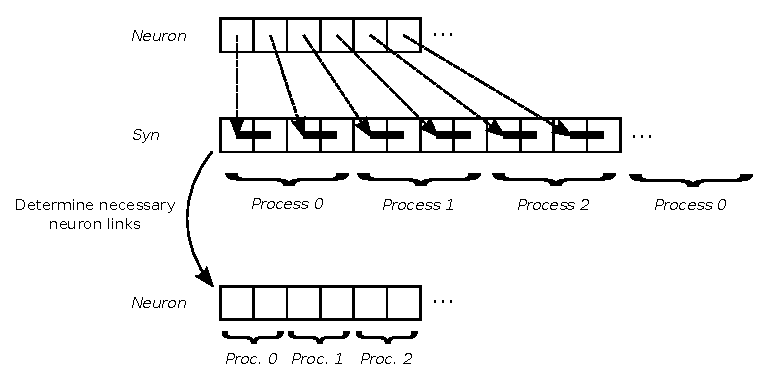
\includegraphics[scale=1.0]{pictures/NeuronLinksRemoving.eps}
\caption{Illustration of the relation of pre-synaptic neuron information to processes.
By reversing the pointer specified in the \emph{neuron} dataset
each entry can be assigned to processes.
Each process can use it to remove unnecessary entries from memory.
}
\label{fig:neuonlinksremoving}
\end{figure}
The distribution of the \emph{syn} dataset is defined.
Each process reads the entries with an offset of $N_{blocksize} * p_{me}$ and
for each iteration it adds a stride of $N_{processes} * N_{blocksize}$  to the offset (e.g see first line in Figure \ref{fig:importsynvis} and \ref{fig:importsynvis2nd}).
Each processes removes all pre-synaptic neuron references, which do not belong to
neurons inside its chunk by reversing the references.

\paragraph{Read step}
From each entry of the block a synapse object is created
(contains pre-synaptic neuron id, post-synaptic neuron id, target neuron process, synapse model parameters)
inside a synapse vector. Then the pre-synaptic neuron ids are integrated into each synapse object.
Each process contains an own vector of synapses.
But most of synapses have to be stored on different processes.
Therefore the process (target process) where the post-synaptic neuron is located is determined (using equation \ref{eq:processfromid})
and integrated.
To send it to the target process, all synapse vectors are sorted by the target neuron process id.
After that \emph{MPI\_Alltoallv} is used to send the synapses from all to all processes.
Each process receives its list of synapses and can use the \emph{NEST} connect function to copy it to its internal data structure.
\begin{figure}[ht!]
\centering
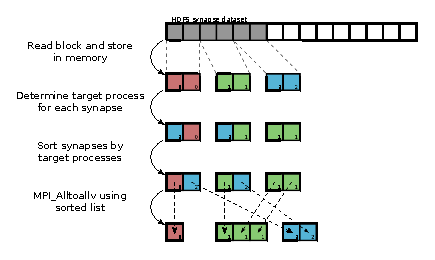
\includegraphics[scale=2.0]{pictures/import_syn_vis.eps}
\caption{Illustration of the first four steps of the algorithm in the first iteration \ref{alg2}.
The first row represents the \emph{syn} dataset on disk.
The following rows represent vectors of synapses per process (represented by the column).
The color of the boxes illustrate the current association.
In the second row the association relates to the position in the \emph{syn} dataset.
Afterwards it relates to the \emph{target process}.
}
\label{fig:importsynvis}
\end{figure}

\begin{figure}[ht!]
\centering

\includegraphics[scale=2.0]{pictures/import_syn_vis_second_it.eps}
\caption{Illustration of the first step of the algorithm in the second iteration \ref{alg2}.
In the second iteration each process reads in the first step the second block of \emph{syn} dataset entries.
A block is specified as the set of read entries per iteration.}
\label{fig:importsynvis2nd}
\end{figure}
\newpage
In the last step of the algorithm, the \emph{connect} function is called iteratively for each synapse.
It is executed multi-threaded.

\paragraph{Connect step}
Each thread calls \emph{connect} for its own synapses iteratively.
Synapse parameters are passed to \emph{connect} function call via a \emph{DictionaryDatum} object.
\emph{DictionaryDatum} is a SLI object for storing a map.
It uses a \emph{Token} mechanism for access elements.
To access entries \emph{Token} objects have to be created and deleted,
which is not thread-safe. It can produce a data race in a static memory pool object of NEST.
Therefore the creation and deletion of the needed \emph{Token} is serialized with mutexes.
Besides the creation of a \emph{DictionaryDatum} object \emph{createDictionaryDatum} creates needed \emph{Token} objects.

In between each thread iterate over all synapses in parallel.
But each thread skips synapses where the post-synaptic is not thread-local.
Thread-locality is given if $t_i$ (see equation \ref{eq:threadfromid}) is equal to the local thread id.
$i$ relates to the target neuron id.
\begin{figure}[ht!]
\begin{lstlisting}[style=cppcode]
#pragma omp parallel default(shared)
{ 
  omp_set_lock(&tokenLock);
  DictionaryDatum* d = createDictionaryDatum();  
  omp_unset_lock(&tokenLock);

  const thread tid = nest::NestModule::get_network().get_thread_id();
      
  for (int i=0;i<synapses_.size();i++) {
    try {
      const thread target_thread = getTargetThread(synapses_[i])
      if (target_thread == tid)
	     singleConnect(synapses_[i], .., target_node, target_thread, ..);
    }
    catch (..) {
      ..
    }
  }
  
  omp_set_lock(&tokenLock);
  delete d;  
  omp_unset_lock(&tokenLock);
}
\end{lstlisting}
\caption{Pseudo code of thread parallel connect function calls.
Parallel region executes code on all available threads.
\emph{singleConnect} function is shown in Figure \ref{fig:singleConnect}.
}
\end{figure}
\emph{singleConnect} assigns the parameters to the \emph{DictionaryDatum} object.
To avoid recreation of \emph{Token} objects a vector of  \emph{Token} pointers is
passed. Applying \emph{set\_{}status} on the passed \emph{Token} objects allow to
insert the current parameters inside the \emph{DictionaryDatum} object without data races.
A for loop iterates over the parameters and copy the values indie the \emph{DictionaryDatum} object.
After that the NEST \emph{connect} function is called with passing besides the source and target
neuron information the \emph{DictionaryDatum} object, weight and delay.
\begin{figure}[ht!]
\begin{lstlisting}[style=cppcode]
void singleConnect(..)
{
  index source = synapse.source_neuron;
  if (NestModule::get_network().is_local_node(target_node)) { 
    for (int i=0; i<param_names.size(); i++) {
      double value = syn.params[i] * facts[i] + offsets[i];
      setValue<double_t>( *v_ptr[i], value );
    }
    NestModule::get_network().connect(.., syn);
  }
  else {
    throw nest::IllegalConnection(..);
  }
}
\end{lstlisting}
\caption{Pseudo code of parameter assignment and NEST internal \emph{connect} function call for a single thread.}
\label{fig:singleConnect}
\end{figure}

\newpage
All in all the implementation make use of available processes and by NEST used cores in the most compute intensive parts.
Figure \ref{fig:ConnectInsideIteration} illustrates the flow of the synapse information between nodes. 
All processes access a single dataset to load a set of it each. Afterwards the synapse information is processed by different steps.
In \emph{Alltoall} the synapse information reordered between the nodes.
So the synapses can be stored in the NEST data structure on the correct process.
\begin{figure}[ht!]
\centering
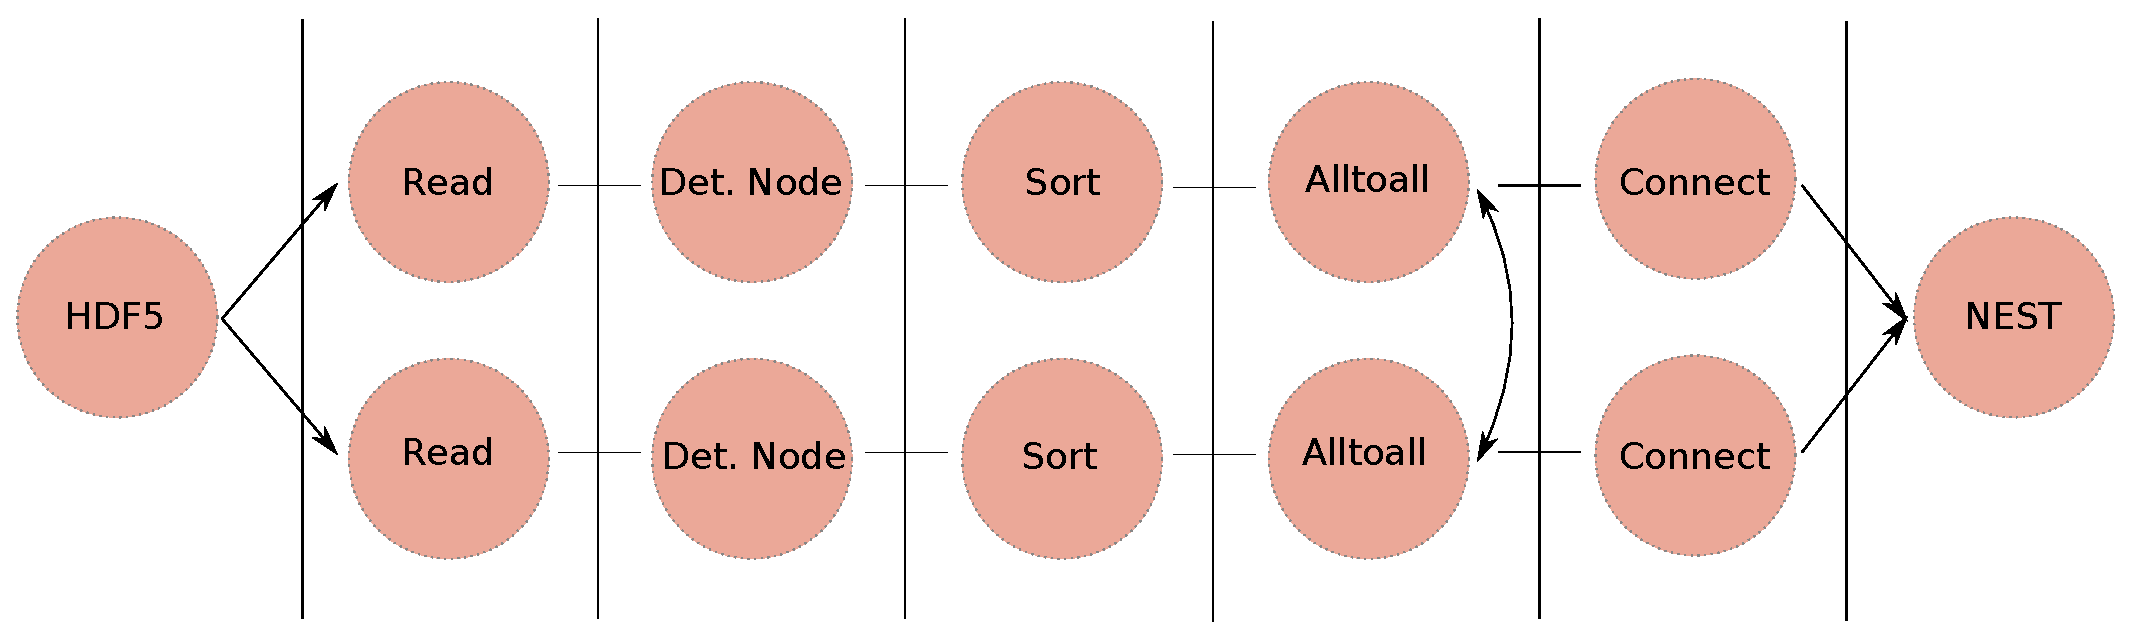
\includegraphics[scale=0.4]{pictures/Connect_inside_iteration.eps}
\caption{Inside iteration parallel work flow}
\label{fig:ConnectInsideIteration}
\end{figure}

\newpage
\section{Memory consumption}
\begin{figure}[ht!]
\begin{tabular}{| l | l | l | l |}
    \hline
    (id) & data structures & memory consumption \\ \hline
    (1) & block in memory & $sizeof(float)*h*p$ \\ \hline
    (2) & target neuron node list & $sizeof(int)*h$ \\ \hline
    (3) & MPI send vectors & $(sizeof(float)*p + sizeof(int)) * h$ \\ \hline
    (4) & MPI recv vectors & $(sizeof(float)*p + sizeof(int)) * \frac{h}{\nu(N)}$ \\ \hline
    \end{tabular}
\caption{$N$: number of processes; $h$: size of block; $p$: number of parameters; $\nu(N)$: distribution coefficient of data}
\end{figure}
The maximum memory consumption is:
\begin{equation}
  M = (sizeof(float)*p + sizeof(int)) * 2h * (1 + \frac{1}{\nu(N)})
  \label{eq:maxmemoryconsumption}
\end{equation}
The block size $p$ is set to $1e6$ for the run on the BG/Q.
It affects the memory consumption and performance loading data from disk.
The implementation could handle different values per process.
But a block size adoption based on memory bottlenecks, is not implemented (see discussion \ref{pAdaption}).